\documentclass{standalone}
\usepackage[utf8]{inputenc}
\usepackage{pgfplots}
\DeclareUnicodeCharacter{2212}{−}
\usepgfplotslibrary{groupplots,dateplot}
\usetikzlibrary{patterns,shapes.arrows}
\pgfplotsset{compat=newest}
\begin{document}
% This file was created with tikzplotlib v0.10.1.
\begin{tikzpicture}

\definecolor{darkgray176}{RGB}{176,176,176}
\definecolor{steelblue31119180}{RGB}{31,119,180}

\begin{axis}[
tick align=outside,
tick pos=left,
title={Derivative step sizes},
x grid style={darkgray176},
xmin=-1.25, xmax=26.25,
xtick style={color=black},
y grid style={darkgray176},
ymin=-0.460332121543895, ymax=10.4981110534069,
ytick style={color=black},
ylabel={$\dfrac{df(x)}{dx}$},
xlabel={step}
]
\addplot [semithick, steelblue31119180, mark=*]
table {%
0 10
1 8
2 6.4
3 5.12
4 4.096
5 3.2768
6 2.62144
7 2.097152
8 1.6777216
9 1.34217728
10 1.073741824
11 0.8589934592
12 0.68719476736
13 0.549755813888
14 0.4398046511104
15 0.35184372088832
16 0.281474976710656
17 0.225179981368525
18 0.18014398509482
19 0.144115188075856
20 0.115292150460685
21 0.0922337203685478
22 0.0737869762948382
23 0.0590295810358706
24 0.0472236648286965
25 0.0377789318629572
};
\end{axis}

\end{tikzpicture}

\end{document}